\documentclass[a4paper,landscape]{slides}
\usepackage{amsmath,amssymb}
\usepackage{kotex}
\usepackage{epsfig}
\usepackage{graphicx}
\usepackage[usenames,dvipsnames]{color}

\usepackage{xcolor}
\usepackage{tikz}
\usepackage[framemethod=TikZ]{mdframed}
\usepackage{environ}
\usepackage{varwidth}
\usepackage[T1]{fontenc}
\usepackage{titlesec, blindtext, color}
\usetikzlibrary{arrows}
%%\usetikzlibrary{matrix}
%%\usetikzlibrary{shadows}


\begin{document}

%%%%%%%%%%%%%%%%%%%%%%%%% Surfaces
\begin{center}
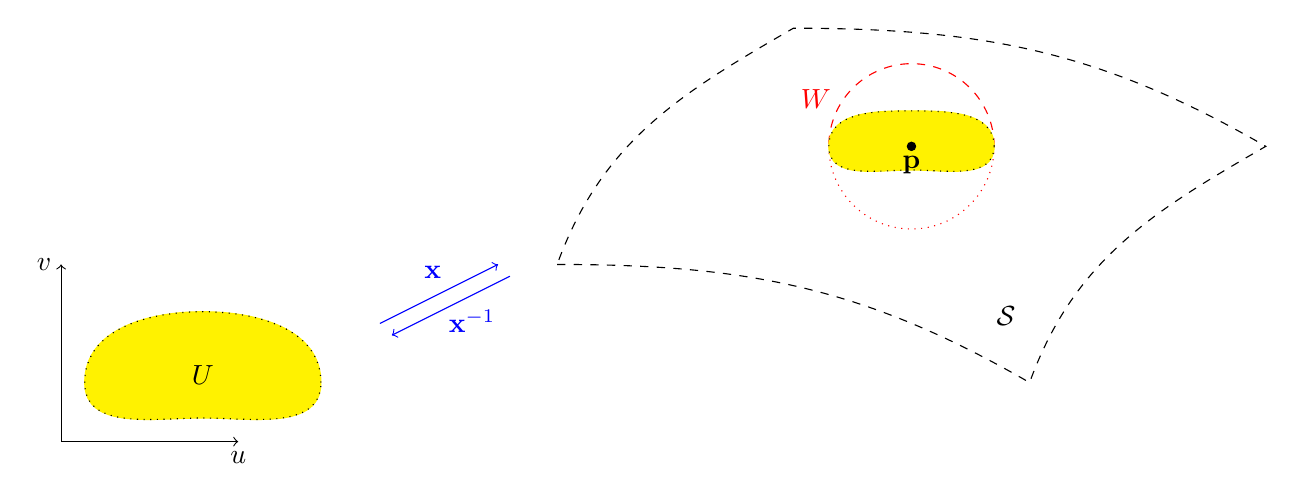
\begin{tikzpicture}[scale=1.5]
 \draw[dashed] (0,0) % S surface 
   to[out=0,in=150] (4,-1) 
   to[out=70,in=210] (6,1) 
   to[out=150,in=0] (2,2)
   to[out=210,in=70] (0,0);
   \draw (3.8,-0.6) node[above] {$\mathcal{S}$};

 \draw[color=red,dashed] (3.7,1) arc (0:180:0.7); % W sphere
 \draw[color=red,dotted] (2.3,1) arc (180:360:0.7);
 \draw[color=red] (2.4,1.4) node[left] {$W$};

 \filldraw[fill=yellow,color=yellow] (3.7,1) % p neighber
   to[out=90,in=0] (3,1.3) 
   to[out=180,in=90] (2.3,1)
   to[out=270,in=180] (3,0.8) 
   to[out=0,in=270] (3.7,1);
 \filldraw[black] (3,1) circle (1pt) node[below] {$\mathbf{p}$};
 \draw[dotted] (3.7,1) 
   to[out=90,in=0] (3,1.3)   
   to[out=180,in=90] (2.3,1)
   to[out=270,in=180] (3,0.8) 
   to[out=0,in=270] (3.7,1);
 
 %%%%%%% surface patch
 \draw[->,color=blue] (-1.5,-0.5) -- (-0.5,0);
 \draw[->,color=blue] (-0.4,-0.1) -- (-1.4,-0.6);
 \draw[color=blue] (-1,-0.3) node[anchor=north west] {$\mathbf{x}^{-1}$};
 \draw[color=blue] (-0.9,-0.2) node[anchor=south east] {$\mathbf{x}$};

 %%%%%%%% uv-plane
 \filldraw[fill=yellow,color=yellow] (-2,-1) 
   to[out=90,in=0] (-3,-0.4) 
   to[out=180,in=90] (-4,-1)
   to[out=270,in=180] (-3,-1.3) 
   to[out=0,in=270] (-2,-1);
 \draw[dotted] (-2,-1) 
   to[out=90,in=0] (-3,-0.4) 
   to[out=180,in=90] (-4,-1) 
   to[out=270,in=180] (-3,-1.3)
   to[out=0,in=270] (-2,-1);
 \draw (-3,-1.1) node[above] {$U$};
 \draw[->] (-4.2,-1.5) -- (-2.7,-1.5) node[below] {$u$};
 \draw[->] (-4.2,-1.5) -- (-4.2,0) node[left] {$v$};
\end{tikzpicture}
\end{center}


%%%%%%%%%%%%%%%%%%%%%% Meusnier
\begin{center}
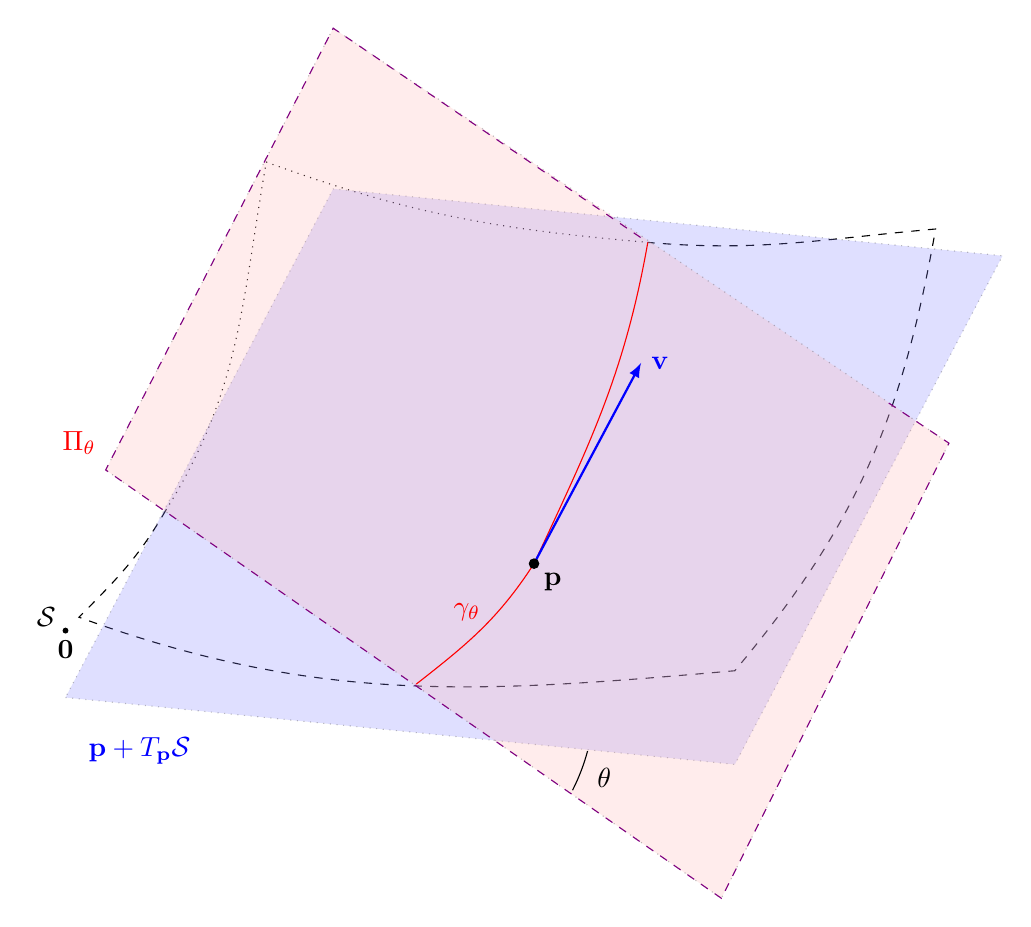
\begin{tikzpicture}[scale=1.7]

   \filldraw[black] (0,0) circle (0.5pt) node[below] {$\small\mathbf{0}$};

 \draw[dashed] (0.75,0.9) % outer of S plane
   to[out=240,in=45] (0.1,0.1) 
   to[out=340,in=185] (5,-0.3) 
   to[out=50,in=260] (6.5,3) 
   to[out=185,in=355] (4.35,2.9);
 \draw[dotted] (0.75,0.9) to[out=58,in=260] (1.5,3.5) to[out=340,in=175] (4.35,2.9);
 \draw (0,0.1) node[left] {$\mathcal{S}$};

 \filldraw[fill=blue!50,dotted,nearly transparent] %tangential plane
 (0,-0.5) -- (5,-1) -- (7,2.8) -- (2,3.3) -- (0,-0.5);
 \draw[color=blue] (0.1,-0.9) node[right] {$\mathbf{p}+T_{\mathbf{p}}\mathcal{S}$};

 \filldraw[fill=red!30,dotted,nearly transparent] %Pi plane
 (2,4.5) -- (6.6,1.4) -- (4.9,-2) -- (0.3,1.2) -- (2,4.5);
 \draw[dashed,color=violet] 
 (6.15,1.7) -- (6.6,1.4) -- (4.9,-2) -- (0.3,1.2) -- (2,4.5) -- (4.35,2.9);
 \draw[color=red] (0.3,1.4) node[left] {$\Pi_\theta$};

 \draw[color=red] (3.5,0.5) to[out=65,in=260] (4.35,2.9); %curve
 \draw[color=red] (3.5,0.5) to[out=237,in=38] (2.62,-0.4);
 \draw[color=red] (3,0) node[above] {$\gamma_\theta$};
 
 \draw[-latex,color=blue,thick] (3.5,0.5) -- (4.3,2) node[right] {$\mathbf{v}$}; %v


 \filldraw[black] (3.5,0.5) circle (1pt) node[anchor=north west] {$\mathbf{p}$}; %p

 \draw (3.9,-0.9) arc (345:333:1.5); %angle
 \draw (3.9,-1.1) node[right] {$\theta$};

\end{tikzpicture}
\end{center}

%%%%%%%%%%%%%%%%%%%%%%%% Riemann sum
\begin{center}
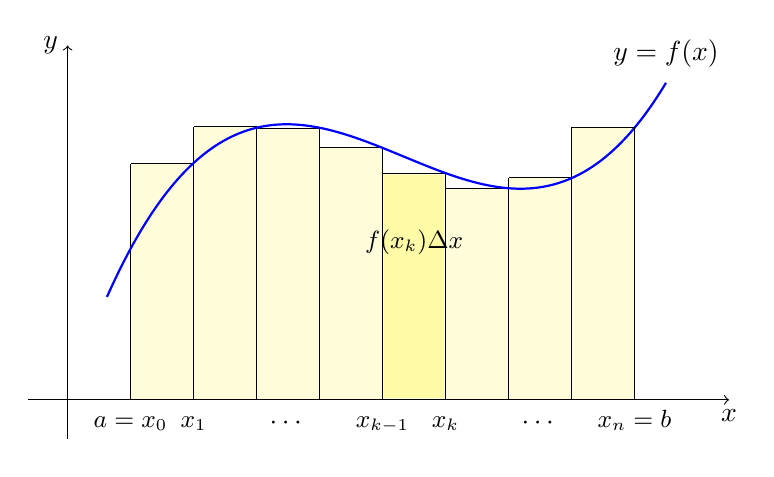
\begin{tikzpicture}
\coordinate (p1) at (0.5,1.4);
\coordinate (p2) at (0.8,1.9); \coordinate (q3) at (0.8,3.0);
\coordinate (p3) at (1.6,3.0); \coordinate (q4) at (1.6,3.47);
\coordinate (p4) at (2.4,3.47); \coordinate (q5) at (2.4,3.45);
\coordinate (p5) at (3.2,3.45); \coordinate (q6) at (3.2,3.2);
\coordinate (p6) at (4,3.2); \coordinate (q7) at (4,2.88);
\coordinate (p7) at (4.8,2.88); \coordinate (q8) at (4.8,2.68);
\coordinate (p8) at (5.6,2.68); \coordinate (q9) at (5.6,2.82);
\coordinate (p9) at (6.4,2.82); \coordinate (q10) at (6.4,3.46);
\coordinate (p10) at (7.2,3.46);
\coordinate (p11) at (7.6,4.1);

\foreach \n in {3,4,5,6,7,8,9,10}
{
\fill[yellow!15] (q\n|-0,0)--(q\n)--(p\n)--(p\n|-0,0)--cycle;
\draw (q\n)--(p\n);
\draw (q\n|-0,0)--(q\n);
\draw (p\n|-0,0) -- (p\n);
}

\fill[yellow!35] (4.02,2.86) -- (4.78,2.86) -- (4.78,0.02) -- (4.02,0.02) -- cycle;

\draw [thick, color=blue, domain=0.5:7.6, samples=200, smooth]
  plot (\x, \x*\x*\x/16-0.8*\x*\x+3*\x);
\draw (p10|-0,0) -- (p10);

\foreach \n/\texto in {2/{a=x_0},3/{x_1},4/{},5/{},6/{x_{k-1}},7/{x_k},8/{},9/{},10/{x_n=b}}
{
  \node[below,text height=1.5ex,text depth=1ex,font=\small] at (p\n|-0,0) {$\texto$};
}

\node at (4.4,2) {\small $f(x_k)\Delta x$};
\draw (2.8,-0.1) node[below] {$\cdots$};
\draw (6,-0.1) node[below] {$\cdots$};

\draw[->] (-0.5,0) -- (8.4,0) coordinate (x axis);
\draw[->] (0,-0.5) -- (0,4.5) coordinate (y axis);

\node[below] at (x axis) {$x$};
\node[left] at (y axis) {$y$};

\node[above] at (p11) {$y=f(x)$};
\end{tikzpicture}
\end{center}

%%%%%%%%%%%%%%%%%%%%%%%%%%%%%% sin & cos
\begin{center}
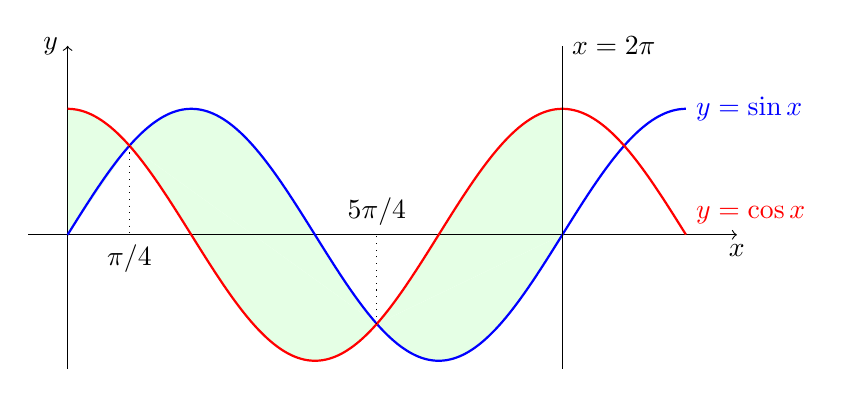
\begin{tikzpicture}
\fill [green!10,domain=0:0.25*pi,variable=\x]
(0,0)-- plot(\x,{1.6*cos(\x r)}) --cycle;
\fill [green!10,domain=0.25*pi:1.25*pi,variable=\x]
(0.75*pi,0)-- plot(\x,{1.6*sin(\x r)}) --cycle;
\fill [green!10,domain=0.25*pi:1.25*pi,variable=\x]
(0.75*pi,0)-- plot(\x,{1.6*cos(\x r)}) --cycle;
\fill [green!10,domain=1.25*pi:2*pi,variable=\x]
(2*pi,0)-- plot(\x,{1.6*sin(\x r)}) --cycle;
\fill [green!10,domain=1.25*pi:2*pi,variable=\x]
(2*pi,0)-- plot(\x,{1.6*cos(\x r)}) --cycle;

\draw[->] (-0.5,0) -- (8.5,0) coordinate (x axis);
\draw[->] (0,-1.7) -- (0,2.4) coordinate (y axis);

\node[below] at (x axis) {$x$};
\node[left] at (y axis) {$y$};

\draw [thick, color=blue, domain=0:2.5*pi, samples=200, smooth]
  plot (\x, {1.6*sin(\x r)}) node[right] {$y=\sin x$};
\draw [thick, color=red, domain=0:2.5*pi, samples=200, smooth]
  plot (\x, {1.6*cos(\x r)}) node[above right] {$y=\cos x$};

\draw (2*pi,-1.7)--(2*pi,2.4) node[right] {$x=2\pi$};
\draw[dotted] (0.25*pi,1.13)--(0.25*pi,0) node[below] {$\pi/4$};
\draw[dotted] (1.25*pi,-1.13)--(1.25*pi,0) node[above] {$5\pi/4$};
\end{tikzpicture}
\end{center}

%%%%%%%%%%%%%%%%%%%%%%%%% 회전체
\begin{center}
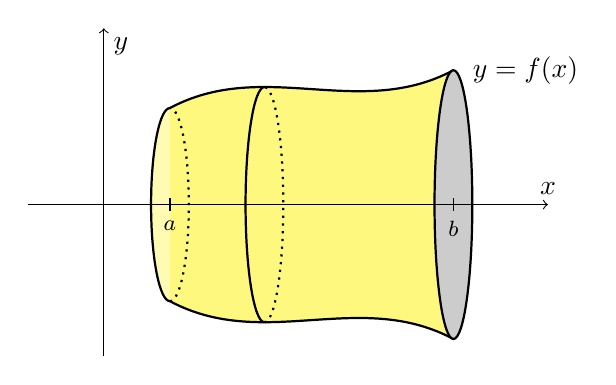
\begin{tikzpicture}[scale=0.8,x=1.5cm,y=0.8cm]
 \fill[fill=yellow,opacity=0.5] (1,0) -- plot[domain=1:4] (\x,{\x*\x*\x/6-5*\x*\x/4+3*\x}) -- (4,0);
 \fill[fill=yellow,opacity=0.5] (1,0) -- plot[domain=1:4] (\x,{-\x*\x*\x/6+5*\x*\x/4-3*\x}) -- (4,0);
 \draw[-,thick,domain=1:4,samples=100] plot (\x,{\x*\x*\x/6-5*\x*\x/4+3*\x}) node[right] { $~y=f(x)$};
 \draw[-,thick,domain=1:4,samples=100] plot (\x,{-\x*\x*\x/6+5*\x*\x/4-3*\x});
 \draw[thick,fill=gray!40] (4,0) circle [x radius =.2 , y radius =2.6666];
 \draw[thick, fill=yellow!30] (1,1.9166) arc(90:270:0.2 and 1.9166);
 \draw[thick,dotted] (1,-1.9166) arc(270:450:0.2 and 1.9166);
 \draw[thick] (2,2.333) arc(90:270:0.2 and 2.333);
 \draw[thick,dotted] (2,-2.333) arc(270:450:0.2 and 2.333);
 \draw[->] (-0.5,0) -- (5,0) node[above] { $x$};
 \draw[->] (0.3,-3) -- (0.3,3.5) node[below right]{ $y$};
 \draw[-] (1,3pt) -- (1,-3pt) node[below] {\footnotesize $a$};
 \draw[-] (4,3pt) -- (4,-3pt) node[below] {\footnotesize $b$};
\end{tikzpicture}
\end{center}

%%%%%%%%%%%%%%%%%%%%%%%%% 회전체
\begin{center}
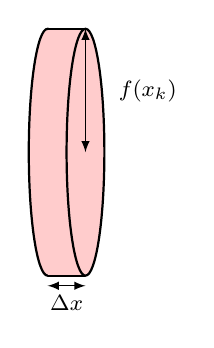
\begin{tikzpicture}[scale=0.8,>=latex,x=1.5cm,y=0.8cm]
  \draw[thick,fill=red!20] (2.3,0) circle [x radius =.2 , y radius =2.449489743];
  \fill[red!20] (2.3,-2.449489743) rectangle (2.7,2.449489743);
  \draw[thick,fill=red!20] (2.7,0) circle [x radius =.2 , y radius =2.449489743];
  \draw[thick] (2.3,2.449489743) -- (2.7,2.449489743);
  \draw[thick] (2.3,-2.449489743) -- (2.7,-2.449489743);
  \draw[<->] (2.3,-2.65) -- (2.7,-2.65) node[below, midway] {\footnotesize $\Delta x$};
  \draw[<->] (2.7,0) -- (2.7,2.449489743) node[right, midway]  {\footnotesize ~~~$f(x_k)$};
\end{tikzpicture}
\end{center}



\end{document} 